\documentclass[12pt,oneside]{book}

\usepackage[bahasa]{babel}

%\usepackage{tgtermes}
%\usepackage[T1]{fontenc}
%\usepackage{libertinust1math}

\usepackage{fontspec}
\setmainfont{TeX Gyre Termes}[
	Numbers = OldStyle,
	Kerning = On
	]

\usepackage{tikz}

\usepackage[all]{nowidow}

\usepackage{multicol}

\usepackage{expex}
   \lingset{
       belowglpreambleskip=-0.2ex,% shrinks the vertical space between the preamble and the top gloss line
       everyglpreamble=\it,
       %everygla=,% removes the default italic formatting of the top gloss line
       aboveglftskip=-0.2ex,% shrinks the vertical space between the aligned lines and the free translation line
       interpartskip=0pt,% vertical space between parts of examples
       glspace=!0pt plus .2em,% improves line breaking by increasing the maximum horizontal space between aligned words
       glrightskip=0pt plus .5\hsize,% improves line breaking by increasing the maximum horizontal space between end of line and the right margin
       aboveexskip=1ex plus .4ex minus .4ex,% vertical space above examples
       belowexskip=1.5ex plus .4ex minus .4ex% vertical space below examples
   }

\usepackage{titlesec}
\titleformat{\chapter}[hang]
{\huge\bfseries}
{\thechapter}
{1em}
{}

\titleformat{\section}
{\normalfont\bfseries}
{\thesection}
{1em}
{}

\titleformat{\subsection}
{\normalfont\bfseries}
{\thesubsection}
{1em}
{}

\titleformat{\subsubsection}
{\normalfont\bfseries}
{\thesubsubsection}
{1em}
{}

\usepackage{fancyhdr}
\fancyhf{}
\renewcommand{\headrulewidth}{0pt}
\fancyfoot[C]{\thepage}

\usepackage{tocbibind} 

\linespread{1.5}

%kamus-part
\usepackage{multicol}
\usepackage{hanging} 

\fancypagestyle{kamus}{
	\fancyhead[L]{\textsc{\rightmark}}
		\fancyhead[R]{\textsc{\leftmark}}
\fancyfoot[C]{\thepage}
}

\newcommand{\arti}[2]{\textit{#1}\ {#2}}
\newcommand{\etym}[1]{\textsc{e}\ {#1}}
\newcommand{\entri}[2]{\markboth{#1}{#1}\textbf{#1}\ {#2}\par}  % Defines the command to print each word on the page, \markboth{}{} prints the first word on the page in the top left header and the last word in the top right

%shorthands
\def\ts{t͡s}
\def\dz{d͡ʒ}
\newcommand\gl[1]{\textsc{\MakeLowercase{#1}}}
\newcommand\krv[1]{\emph{#1}}

%basic-infos

\begin{document}
\frontmatter

\thispagestyle{empty}
\vspace*{\fill}

\begin{figure}[h]
	\centering
	
\includegraphics[width=0.6\textwidth]{media/cover.jpg}
\end{figure}

\begin{center}
	{\huge Bahasa Krewi}

	{\large seven}

	\today
\end{center}
\clearpage

\pagestyle{fancy}
\tableofcontents
\listoffigures

\mainmatter
\chapter{Pengantar}
\section{Latar Belakang Eksternal}
Bahasa Krewi adalah sebuah basareka yang penulis kembangkan dalam frekuensi yang tidak konsisten sejak Desember 2012. Tidak ada tujuan spesifik yang penulis tuju dalam membangun Bahasa Krewi. Oleh karena itu, bahasa ini terlepas dari konteks budaya tertentu di dunia dan mengambil dimensi \emph{a priori} dengan penutur dan latar belakang kultural yang baru.

\section{Kredan dan Orang-orangnya}
Kredan merujuk pada lahan yang diketahui dalam Saga Kredan yang membentang sedari lahan arid subtropis di selatan hingga hutan hujan di utara dan dibatasi oleh rantai tanah tinggi Pegunungan Weurzan di barat dan Lautan Ilwehe di tenggara. Leiri Kieuwel, salah satu populasi inti dalam Saga Kredan, adalah salah satu dari tiga populasi yang telah lama terpisah dari rombongan asalnya. Orang-orang Leiri datang dari tanah yang jauh lebih selatan yang dalam Saga Kredan dikenal secara sederhana sebagai Tanah Tua. Alasan migrasi penuh Leiri tidak diketahui secara pasti, tetapi diketahui dengan pasti Leiri terusir karena Bencana Dingin yang meliputi seluruh Tanah Tua dengan menurunnya temperatur rata-rata secara drastis di sebagian besar pemukiman Leiri. Rombongan Leiri tiba di tanah Kredan kira-kira sekitar lima--enam generasi lalu di sebuah titik di tanah arid yang kini terletak di jantung Kenaharan Majal.

Majal, dengan iklim arid dan rata-rata hujan tahunan yang minim, dikenal sebagai tanah yang kurang subur. Populasi Majal hampir sepenuhnya bergantung pada hasil hewani. Oleh karena itu, untuk menjamin keberlangsungan Leiri, populasi penduduk Majal dibagi menjadi empat dengan tiga di antaranya pergi berkelana meninggalkan Majal. Dengan menggunakan Puncak Weurza sebagai kompas, satu dari tiga kelompok pengelana tiba di tanah di utara yang lebih subur. Tanah subur tersebut didukung dengan ekosistem Estuari Kieuwel yang, pada masa itu, dihuni oleh beberapa kelompok etnis yang beragam. Pengelana Leiri tersebut kemudian melakukan kontak intensif pertama mereka oleh orang-orang yang Leiri sebut sebagai Ceurgan. Leiri tinggal bersebelahan dengan Ceurgan untuk waktu singkat hingga akhirnya mereka dihadiahkan tempat untuk bermukim di barat Mulut Kieuwel.

Komunitas Leiri Kieuwel, berawal dari pemukiman sederhana di tepian sungai-sungai Kiehai, berkembang pesat melebihi penduduk asli Kredan berkat satu hal yang mereka tidak miliki. Leire Kieuwel menarik sistem tulisan Jeren, yang sebelumnya dianggap sakral, ke alam profan dan menginternalisasikannya ke kehidupan sehari-hari. Sungai-sungai di Kiehai adalah pintu utama ekonomi sekaligus jalur transportasi pemukiman-pemukiman di tanah tinggi menuju suku-suku di muara. Didampingi dengan makin bergantungnya budaya Leiri Kieuwel dengan Jeren, Lejar berdiri tegak sebagai titik temu dan pengarah arus perdagangan dari hulu ke hilir. Kemantapan laju perkembangan Lejar berubah drastis kala pamor Majal yang menaik sebagai \emph{nahar} `pusatnya ilmu' tiba di telinga-telinga priyayi-priyayi Zeshtir di utara. Keberadaannya membuat Lejar tumbuh sebagai titik hubung antara empat penjuru yang sepenuhnya oral. 

\begin{figure}[]
	\centering
	\fbox{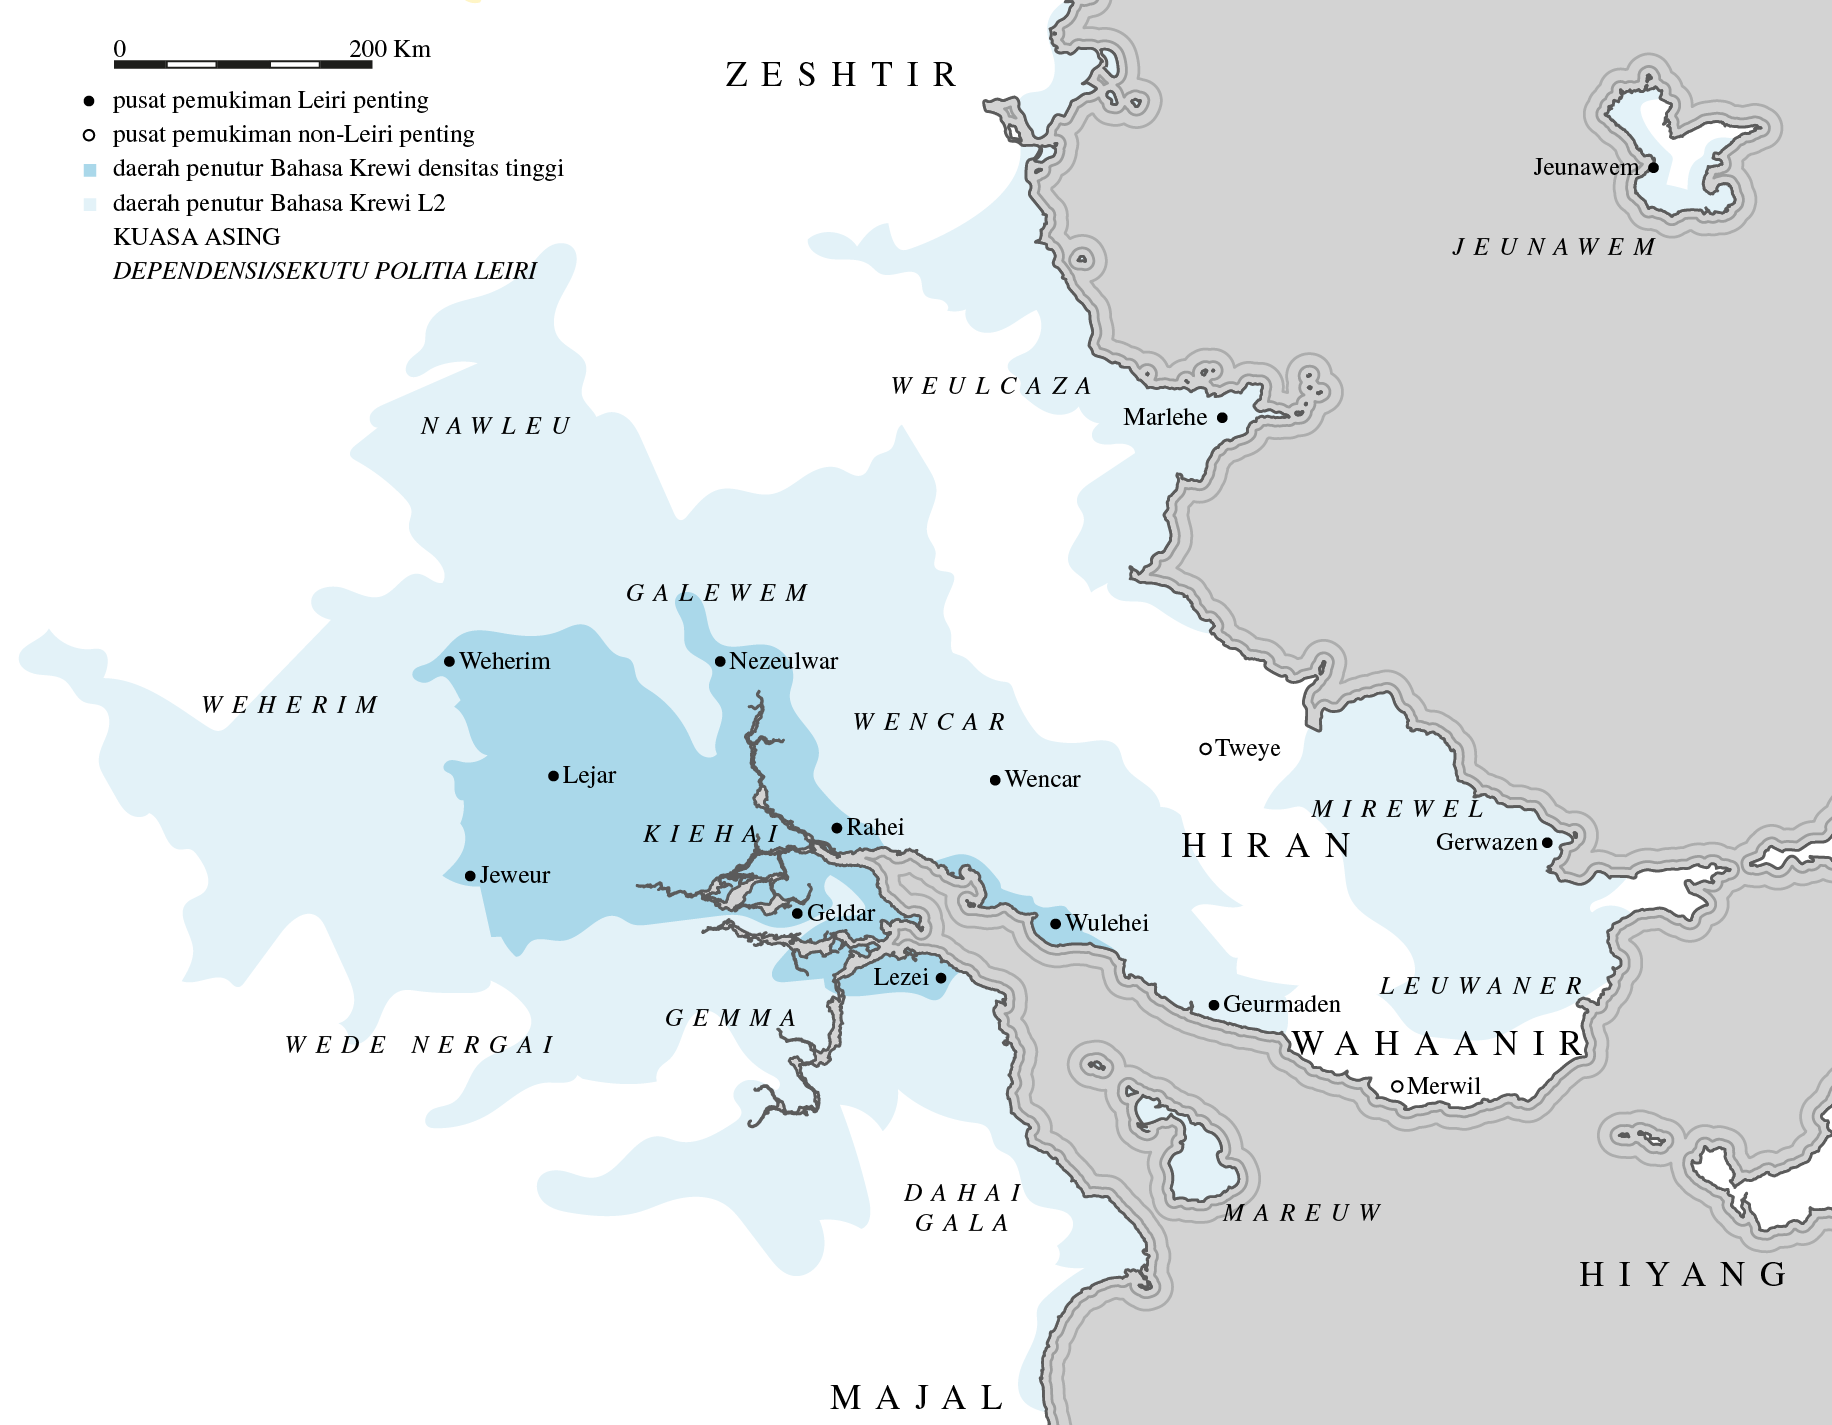
\includegraphics[width=\textwidth]{media/krewimap1.png}}
	\caption{Persebaran penutur Bahasa Krewi.}
	\label{fig:1}
\end{figure}

Tingginya pamor Lejar memudahkan terbentuknya rentang kuasa Leiri Kieuwel yang menembus sungai-sungai Kiehai. Leiri Kieuwel, ketimbang membumihanguskan, dengan mudah membentuk aliansi dan hubungan dagang langsung pada pemukiman-pemukiman di sekitarnya. Kini, pada Saga Kredan, jaring-jaring kuasa Leiri Kieuwel merentang sedari Weherim di barat hingga pemukiman penambang azurit di Jeunawem. Jeunawem, dikenal sebagai `bandul biru Kredan', telah lama disebut-sebut sebagai tanah yang suci bagi penduduk asli Kredan. Tanah suci yang dikuasai oleh kuatnya tulisan membuat Lejar sebagai penghubung budaya dan perdagangan semakin kuat.

Populasi Lejar kian signifikan dengan aliansi dengan pendatang lain yang kini dihuni oleh Orang-orang Hiyang di timur jauh. Lautan dangkal yang menghubungkan Jeunawem dan tanah induk dikenal sebagai penghambat utama dalam eksploitasi azurit yang maksimum. Hiyang mengenalkan komunitas Lejar pada sekunar-sekunar yang lebih besar dengan daya berlayar yang lebih baik ketimbang kapal kecil Leiri. Hiyang membuka jalan untuk perjalanan memutar menuju Jeunawem melewati Kihaba, ibu kota Hiyang, menuju Jeunawem dan sebaliknya. Interaksi tersebut memakmurkan keduanya. 


\section{Bahasa Krewi}
Bahasa Krewi adalah salah satu dari subgrup Bahasa-bahasa Eiwem yang datang dari Tanah Tua. Rumpun subgrup Bahasa-bahasa Eiwem di Kredan mencakup kontinuum dialek sedari Krewi di utara hingga komunitas barat daya Majal. Secara umum kontinuum tersebut dapat dibagi menjadi lebih dari 6 bahasa. Bahasa Krewi umum dipertuturkan di pemukiman Leiri Kieuwel densitas tinggi di antaranya di wilayah Lejar, Kiehai, Gema, dan beberapa daerah selatan Semenanjung Ceura.

Bahasa Krewi juga dipertuturkan sebagai bahasa pemersatu di sebagia besar dependensi Lejar dan sebagai bahasa diplomasi antara Politia Leiri dan Kahari Hiyang.

\chapter{Fonologi}
WIP


\chapter{Kategorisasi leksikon}
\section{Kelas terbuka}
Terdapat banyak akar kata yang dapat berfungsi nominal atau pun verbal tanpa memerlukan perubahan morfologis tertentu selain pengubah peran semantik.

\pex
\a
\begingl
\gla deure ge twahe //
\glb {\sc p}.kepemilikan {\sc 1s} musuh //
\glft `Aku memiliki musuh' //
\endgl
\a
\begingl
\gla twahe ge lemalai //
\glb {\sc a}.musuh {\sc 1s} pemuka\_agama //
\glft `Aku memusuhi pemuka agama' //
\endgl
\a
\begingl
\gla ger we twahe jeun zawe //
\glb {\sc hab} {\sc p.}ada musuh air minyak // 
\glft `air dan minyak selalu bermusuhan' //
\endgl
\xe

Pada contoh (\lastx a), kata \emph{twahe} `musuh' digunakan sebagai nomina, tetapi pada (\lastx b) \emph{twahe} digunakan sebagai verba dengan bentuk yang sama. Selain keduanya, (\lastx c) menunjukkan \emph{twahe} digunakan sebagai adjektiva. Berikut dijelaskan beda di antara ketiganya.

\section{Kelas tertutup}
\subsection{Adverbia}
\ex Adverbia temporal\par\nobreak\medskip 
\quad\vbox{\halign{
	#\hfil& \hskip3em #\hfil& \hskip3em #\hfil\cr
	\noalign{\smallskip}
	\emph{wajeu}& masa-\textsc{def}& `kini'\cr
	\emph{wahir}& masa-\textsc{dem.prox}& `tadi'\cr
	\emph{lewir}& & `selanjutnya'\cr
	\emph{wareuw}& masa-\textsc{dem.dist}& `lampau'\cr
	\emph{gargal}& & `masa yang akan datang'\cr
}}\xe

\ex Adverbia epistemik\par\nobreak\medskip
\quad\vbox{\halign{
	#\hfil& \hskip3em #\hfil& \hskip3em #\hfil\cr
	\noalign{\smallskip}
	\emph{euja}& & `tiba-tiba'\cr
}}\xe

\ex Adverbia frekuentatif\par\nobreak\medskip
\quad\vbox{\halign{
	#\hfil& \hskip3em #\hfil& \hskip3em #\hfil\cr
	\noalign{\smallskip}
	\emph{jeuran}& & `jarang`\cr
	\emph{gang}& & `kadang-kadang'\cr
	\emph{zemir}& & `sering'\cr
}}\xe

\ex Adverbia derajat\par\nobreak\medskip
\quad\vbox{\halign{
	#\hfil& \hskip3em #\hfil& \hskip3em #\hfil\cr
	\noalign{\smallskip}
	\emph{waheuw}& & `hanya saja, hanya ini`\cr
	\emph{ganewer}& & `hampir'\cr
	\emph{jahai}& & `sangat'\cr
	\emph{gazew}& &`terlalu'\cr
}}\xe

Seluruh adverbia umumnya diutarakan sebelum verba.

\ex
\begingl
\gla gargal tlewi Mari //
\glb akan {\sc a}.tiba {\sc nama} // 
\glft `Mari akan datang' //
\endgl
\xe

\ex
\begingl
\gla euja bahal //
\glb tiba-tiba {\sc p}.hujan // 
\glft `Tiba-tiba turun hujan' //
\endgl
\xe

\ex
\begingl
\gla jeuran dareun cahewe//
\glb jarang {\sc p}.sepi tempat\_luas-{\sc def} // 
\glft `Lapangan ini jarang sepi' //
\endgl
\xe

\ex
\begingl
\gla waheuw we geher//
\glb hanya {\sc a}.ada {\sc 2s} // 
\glft `Hanya ada kamu' //
\endgl
\xe

\subsection{Pronomina}
WIP

\subsection{Demonstratif}
WIP

\subsection{Angka}
Angka memiliki bentuk penuh dan bentuk klitika.

\ex \vtop{\labels\halign{#\hfil& \hskip3em #\hfil& \hskip3em #\hfil\cr
	&bentuk penuh& klitika\cr
	1& \emph{gahi}& \emph{gi}\cr
	2& \emph{rehi}& \emph{ri}\cr
	3& \emph{zergang}& \emph{zan}\cr
	4& \emph{erma}& \emph{er}\cr
	5& \emph{leul}& \emph{leul}\cr
	6& \emph{baleuw}& \emph{bal}\cr
	7& \emph{meuneu}& \emph{meum, meu}\cr
	8& & \cr
	9& & \cr
}}\xe

\subsection{Penggolong}
WIP

\subsection{Interogatif}
WIP

\subsection{Konjungsi}
WIP


\chapter{Sintaks}
\section{Kalimat Sederhana}
Kalimat Bahasa Krewi sederhana harus terdiri dari verba dengan konstituen lain dianggap opsional. Berarti, sebuah verba mandiri dapat memiliki arti dengan sendirinya. Ingat bahwa, pada dasarnya, verba selalu mengandung makna penderita.

\ex
\begingl
\gla lacei //
\glb {\sc p}.sakit // 
\glft `(dilanda) sakit' //
\endgl
\xe

Pada kalimat dengan peran subjek yang jelas, subjek diletakkan setelah deklarasi verba. Peran semantik subjek sebagai pelaku ditentukan secara eksplisit dengan konjugasi verba menjadi verba 2.

\pex
\a
\begingl
\gla cehe mer krezei //
\glb {\sc p}.geletar {\sc 3s} {\sc caus}-hawa\_dingin //
\glft `dia gemetar karena kedinginan' //
\endgl
\a
\begingl
\gla ceuhe mer krezei //
\glb {\sc a}.geletar {\sc 3s} {\sc caus}-hawa\_dingin //
\glft `dia bergoyang karena hawa dingin' //
\endgl
\xe

Beberapa verba memiliki bentuk tak umum untuk verba 2-nya.

\pex
\a
\begingl
\gla leuha mer //
\glb {\sc p}.jatuh\_ke\_bawah {\sc 3s} //
\glft `dia tergelincir' //
\endgl
\a
\begingl
\gla trahe mer //
\glb {\sc a}.jatuh\_ke\_bawah {\sc 3s} //
\glft `dia (men)jatuh(kan dirinya sendiri)' //
\endgl
\xe

Pada kalimat dengan dua objek atau lebih, konstituen diletakkan sembarang dengan valensi ditentukan dengan kelas kata yang dikandungnya. Kelas kata Bahasa Krewi dikelompokkan berdasarkan derajat kehidupan yang dimilikinya. Secara berurutan dari yang paling `hidup' hingga `mati' adalah: ego; saudara tunggal; saudara jamak; khalayak tunggal; khalayak jamak; non-leiri (hewan/tumbuhan); kuasa alam; peralatan atau benda buatan; benda mati; dan, abstrakta.

\pex
\a
\begingl
\gla lahai gihe Wele //
\glb {\sc a}.beri ikan {\sc nama} //
\glft `Wele membagikan ikan' //
\endgl
\a
\begingl
\gla lahai gihe Wele leima //
\glb {\sc a}.beri ikan {\sc nama} khalayak //
\glft `Wele membagikan orang-orang ikan' //
\endgl
\xe

Pada beberapa verba, valensi digunakan untuk memberi kesan purposif dengan kelas terendah sebagai objek langsung.

\pex
\a
\begingl
\gla kieuze kraweu Wele gihangar //
\glb {\sc a}.baca buku {\sc nama} peliharaan-{\sc attr.3s} //
\glft `Wele membacakan Gihang buku' //
\endgl
\a
\begingl
\gla zeuwer weuma Wele galwere //
\glb {\sc a}.warna rumah {\sc nama} bebatuan //
\glft `Wele menghias (lahan) bebatuan (dengan) rumah' //
\endgl
\xe

\backmatter
\chapter{Kamus}
\section{Cara Pemakaian}
---dust---
\clearpage

\pagestyle{kamus}
\begin{multicols}{2}
	\begin{hangparas}{1.5em}{1}
		\entri{cekrewim}{\arti{v}{membuat tidak nyaman, membuat tidak aman; mengagitasi} \arti{n}{ketidakamanan, ketidaknyamanan, kegelisahan}}
		\entri{gahang}{\arti{n}{permainan lompat tali}}
		\entri{jeuheng}{\arti{v}{menyebabkan kekacaubalauan, membuat kacau, membuat berantakan; mengacak; membuat gaduh; merusak tatanan} \arti{n}{kekacauan, ketidakteraturan; kebingungan, kekacaubalauan; kegaduhan; reruntuhan, ceceran sampah} \arti{adj}{kacau balau, berantakan; tidak seharusnya (hanya dalam penggunaan jamak)}}
		\entri{kwihar}{\arti{v}{memotong dengan kapak; menghantam dan memotong kasar} \arti{n}{kapak} \etym{Wah. \textit{gueyhar} `kapak kayu', kapak kecil untuk memotong dan menghaluskan kayu. Sebagai tukang yang berani, beberapa pengelana bercerita mengenai orang-orang Wah. yang meneror dan menyerang karavanir dan rakyat dengan kapak kayu.}}
		\entri{leuwgeung}{\arti{v}{menyelesaikan (masalah), mencari solusi; memahami masalah} \arti{n}{pemahaman, kesadaran akan masalah, pengertian; persetujuan}}
		\entri{marleje}{\arti{v}{memanggul beban} \arti{n}{penahan, tiang (bangunan)}}
		\entri{rehel}{\arti{v}{memanggul beban dengan pundak} \arti{n}{tongkat panggul}}
		\entri{zehedi}{\arti{v}{menyambungkan, menggabungkan, mengikat; mengencangkan (dengan tali); berlabuh} \arti{n}{ikatan, simpul; koneksi, ikatan sosial, kesetiaan}}
\end{hangparas}

\end{multicols}


\end{document}
